\documentclass[12pt,a4paper]{article}

\usepackage{graphicx}
\usepackage{abstract}
\usepackage{hyperref}
\usepackage{listings}
%\usepackage{amssymb}
%\usepackage{indentfirst}

\graphicspath{ {./images/} }
\renewcommand{\abstractname}{\large{Timestamps}}

\setlength{\parindent}{0.5in}

\title{CPSC 335 | Lecture \#4}
\author{Chris Nutter\thanks{Dedicated to @QuesoGrande a.k.a. Jared D.}}

% --> Here we go, satellite radio, y'all get hit with a...

\begin{document}

\maketitle

\begin{abstract}
    \noindent
    \begin{center}\textbf{09/21/2020 - 07:27:25 PM}\end{center}
        \textbf{MIDTERM NEXT WEEK!}\\
\end{abstract}

\tableofcontents

% -->

\section{Lecture}
    
    \begin{figure}[!hbtp]
        \centering
        \fbox{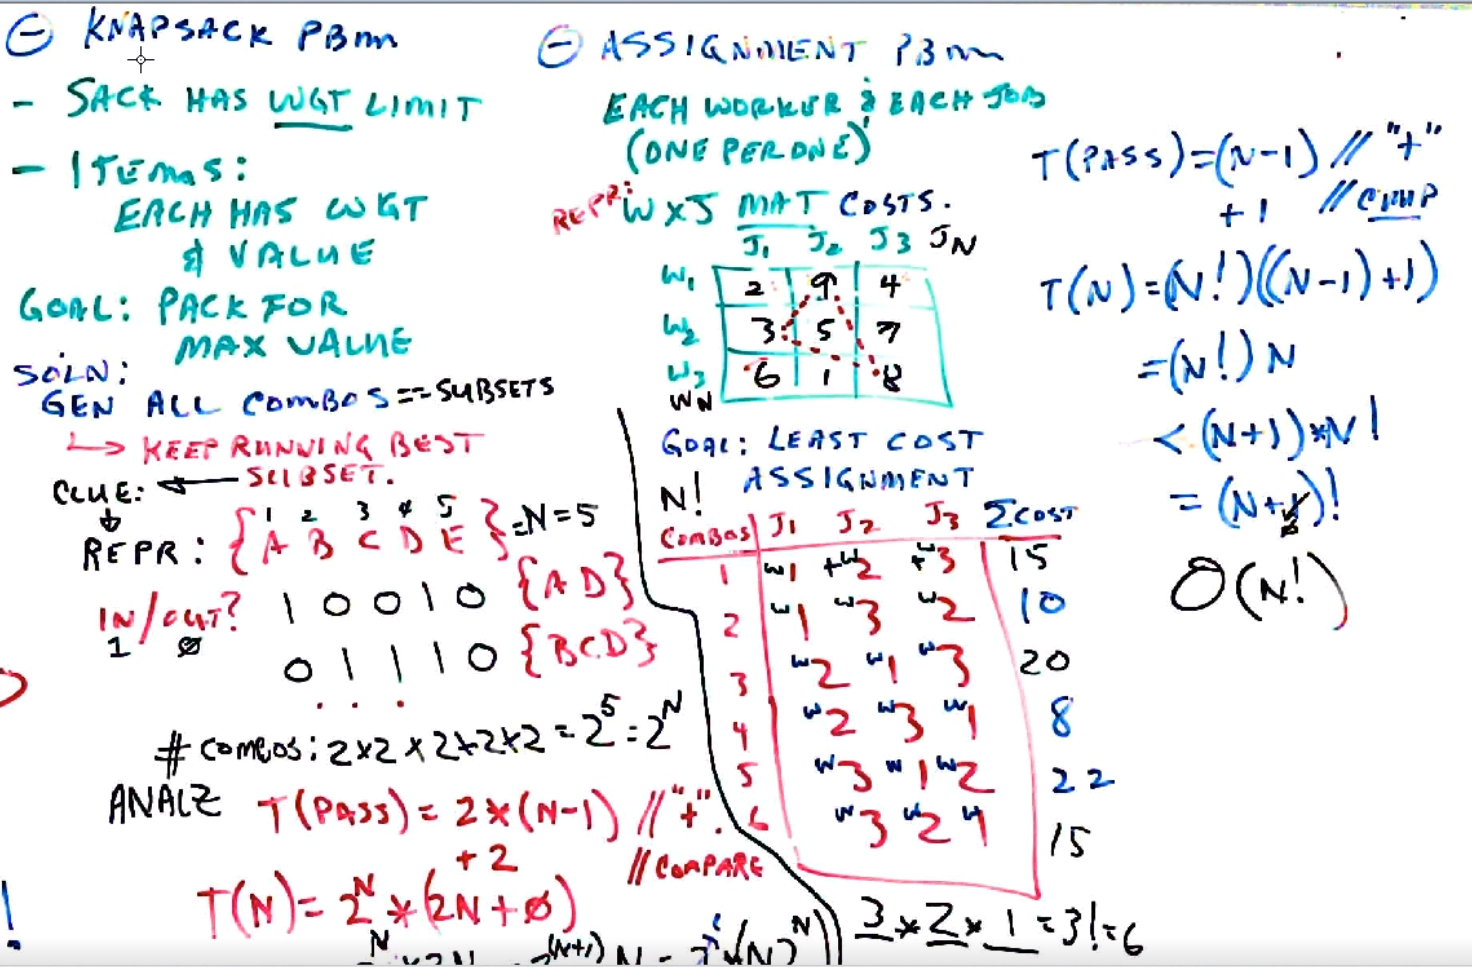
\includegraphics[width=13.8cm]{knapsack.png}}
        \caption{Knapsack Problem}
    \end{figure}

    \begin{figure}[!hbtp]
        \centering
        \fbox{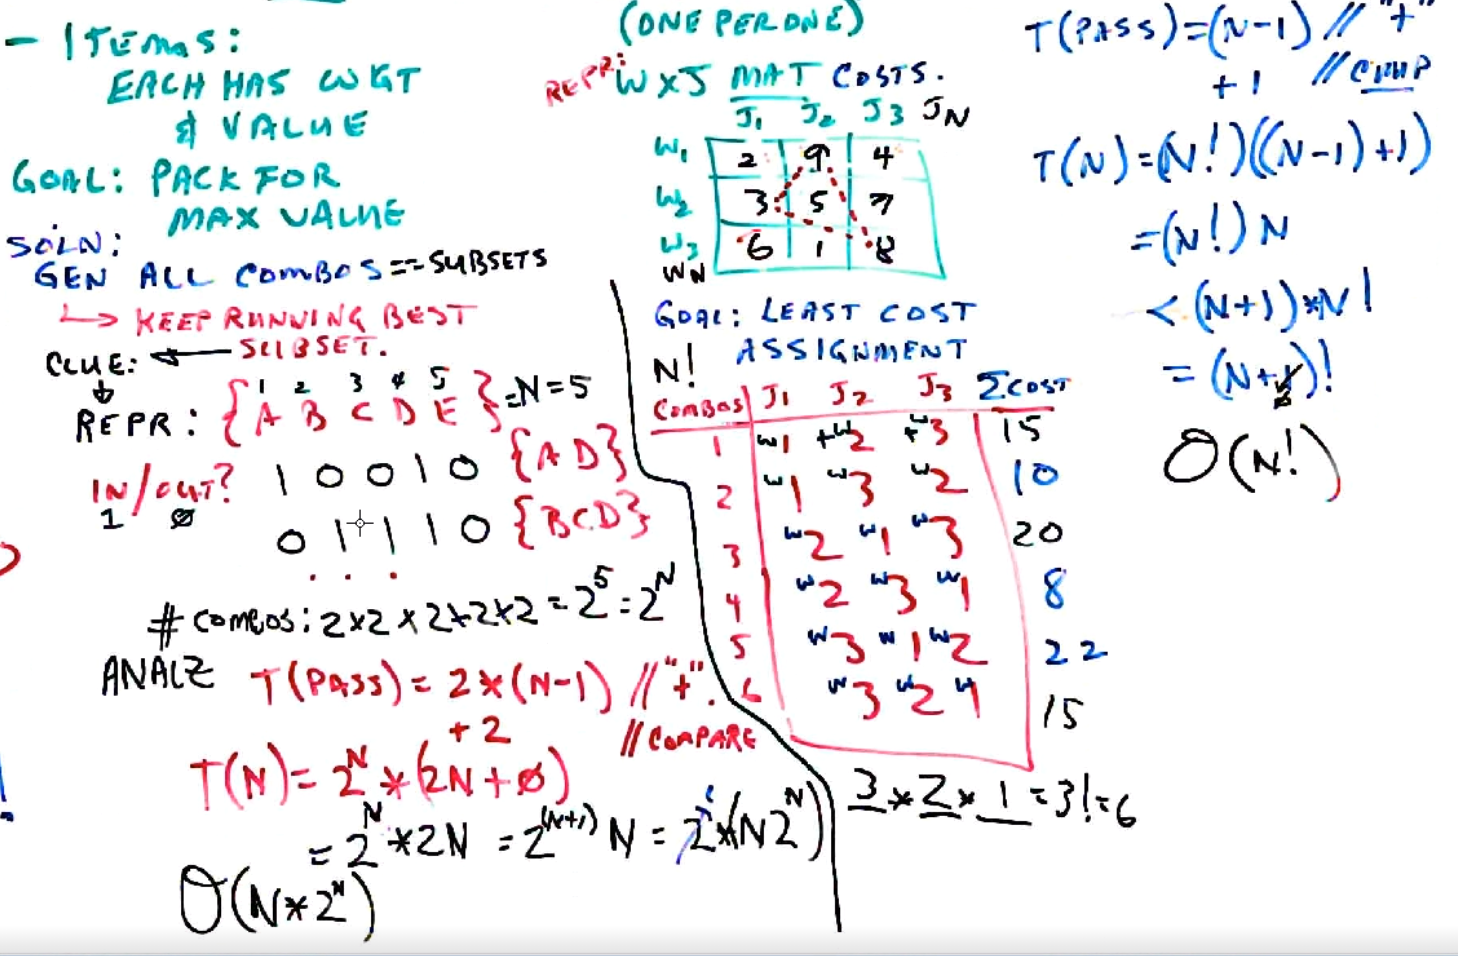
\includegraphics[width=13.8cm]{knapsack-cont.png}}
        \caption{Knapsack Problem (\emph{cont.})}
    \end{figure}

    \begin{figure}[!hbtp]
        \centering
        \fbox{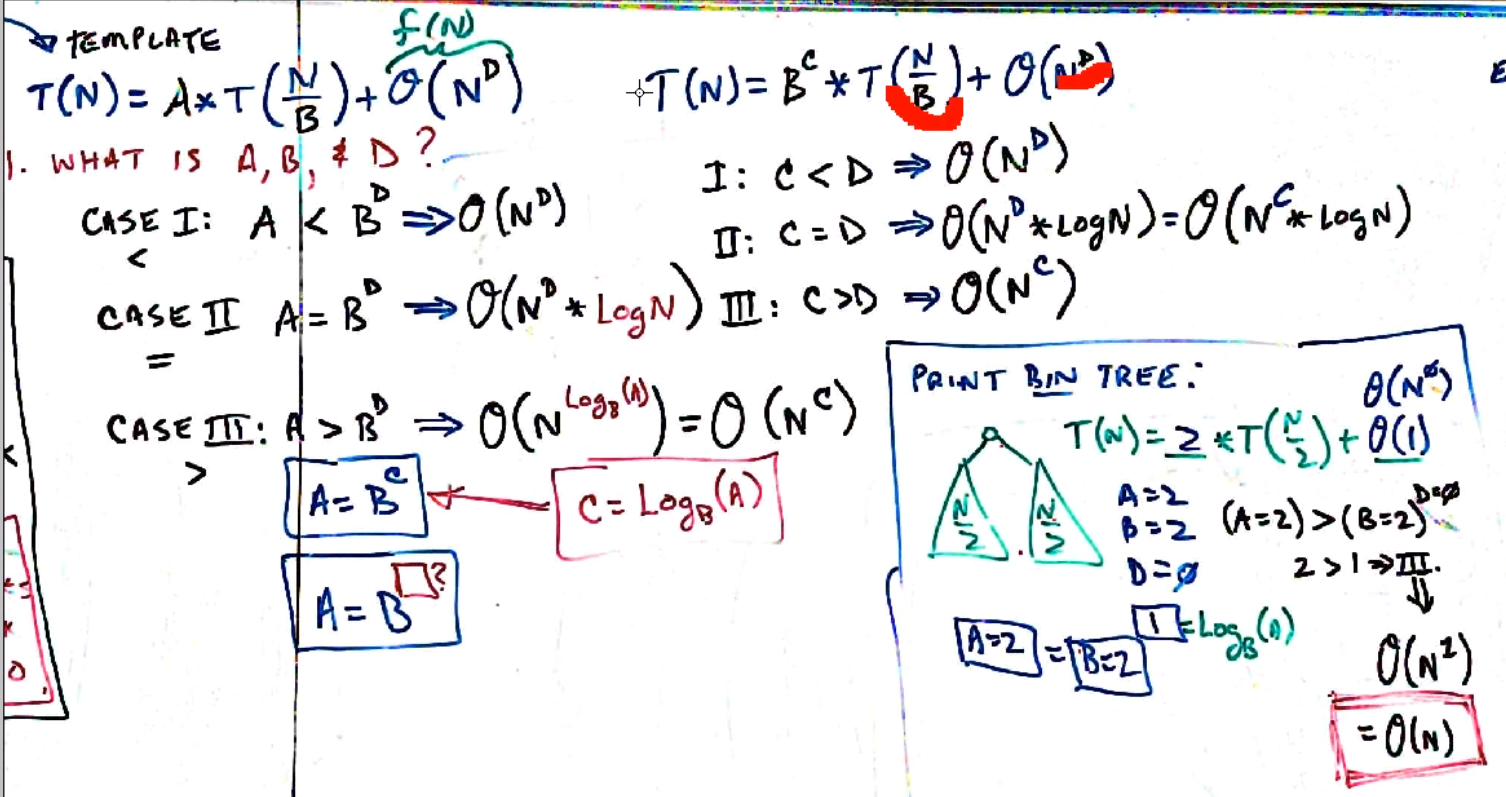
\includegraphics[width=13.8cm]{o(nd).png}}
        \caption{$O(N^{D})$}
    \end{figure}

    \begin{figure}[!hbtp]
        \centering
        \fbox{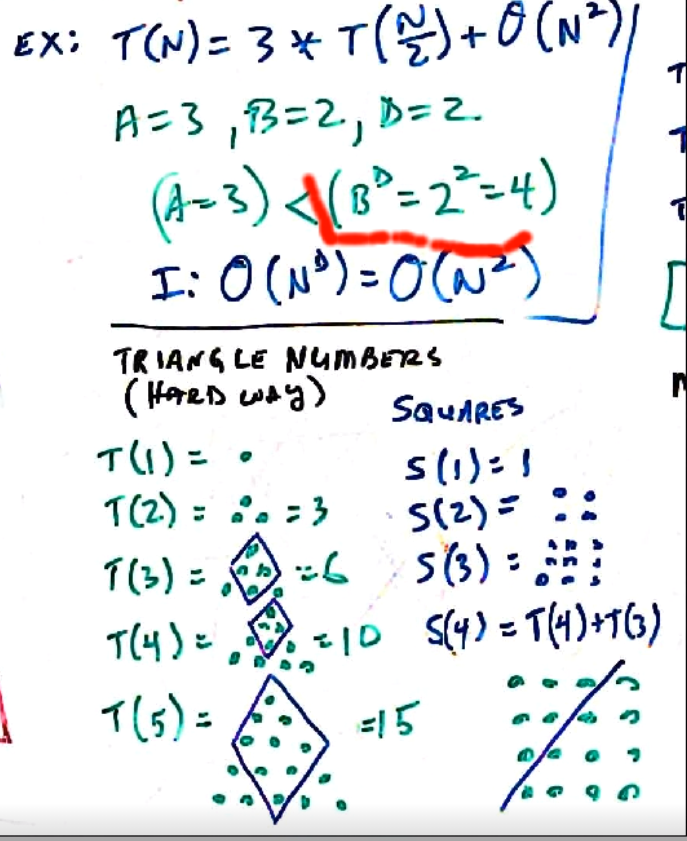
\includegraphics[width=13.8cm]{triangle-num.png}}
        \caption{Triangle Numbers Problem}
    \end{figure}

    \begin{figure}[!hbtp]
        \centering
        \fbox{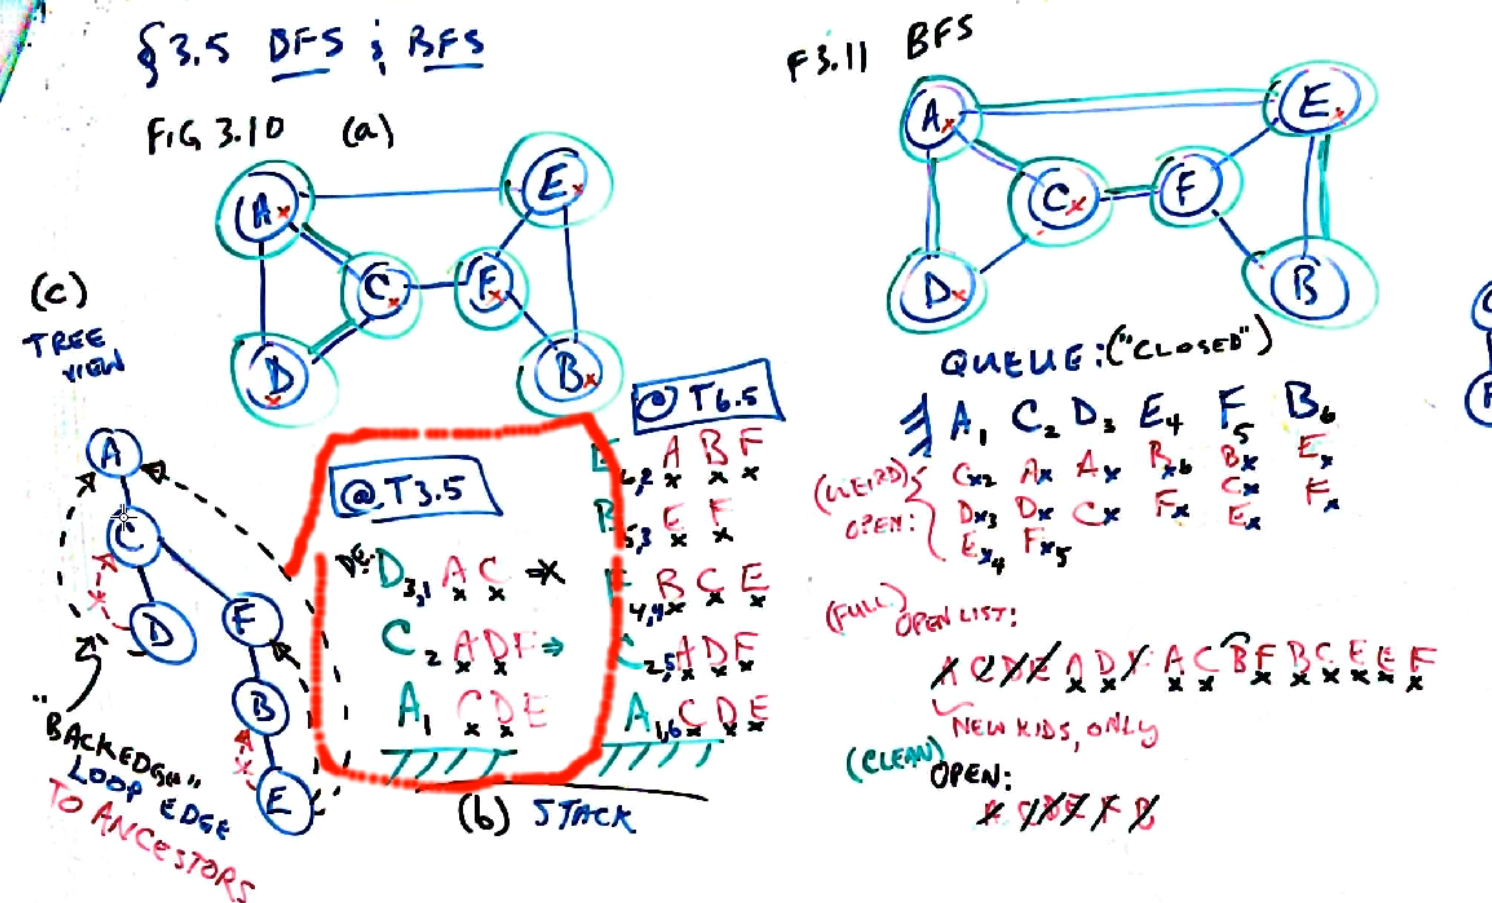
\includegraphics[width=13.8cm]{dfs3.1.png}}
        \caption{Depth First Search | Fig. 3.10}
    \end{figure}


    \begin{figure}[!hbtp]
        \centering
        \fbox{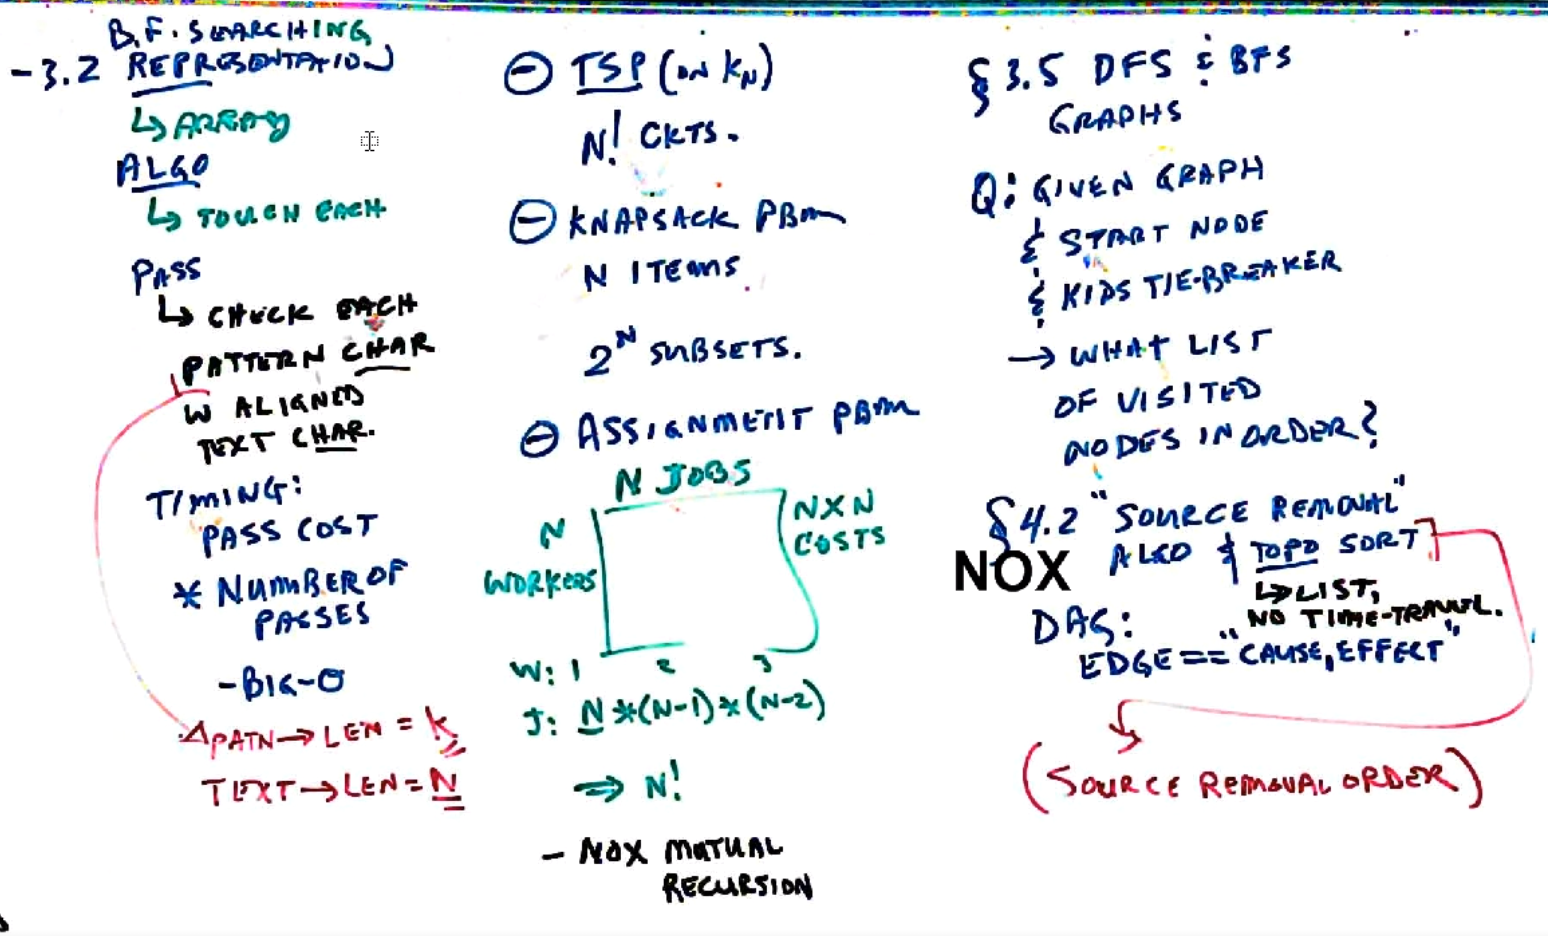
\includegraphics[width=13.8cm]{bfs.png}}
        \caption{Breadth First Search}
    \end{figure}

\newpage
\section{Review}
    
    \begin{figure}[!hbtp]
        \centering
        \fbox{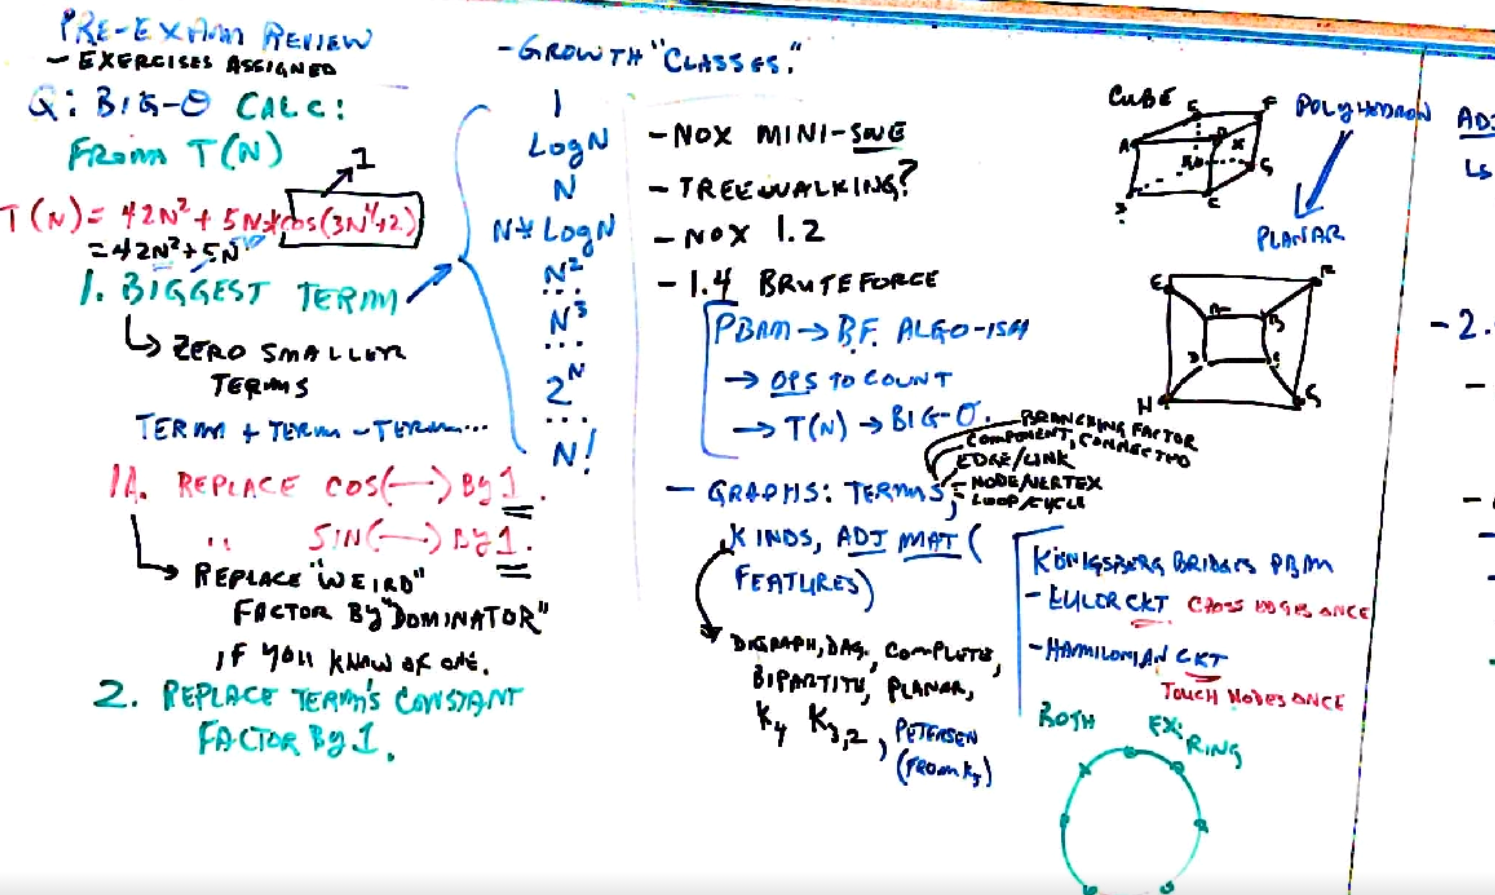
\includegraphics[width=13.8cm]{review-1.1.png}}
        \caption{Review Pt. 1}
    \end{figure}



\end{document} 
